\subsection{Pagina de registo}

Esta página permite que os utilizadores registados não autenticados, efetuem autenticação para poderem aceder a todas as funcionalidades do sistema.\\

Depois da referida autenticação, os utilizadores serão direcionados para o painel do aluno ou docente, dependendo do tipo de utilizador que este indicou no registo.

Nesta página os utilizadores não autenticados podem regressar à página inicial, ao carregar no logótipo do sistema, aceder à página de registo ou recuperar a \textit{password} esquecida.

O utilizador é notificado com mensagens de erro explicitas quando falhar o autenticação, por erro nos campos pedidos ou por falta de registo.

Para esta página procurou-se um \textit{design} simples, onde o utilizador pode concentrar-se exclusivamente na funcionalidade pretendida, a autenticação.\\

Na Figura~\ref{fig:sign_in} pode ser consultada uma imagem demonstrativa da página desenvolvida.\\

\begin{figure}[H]
  \centering
  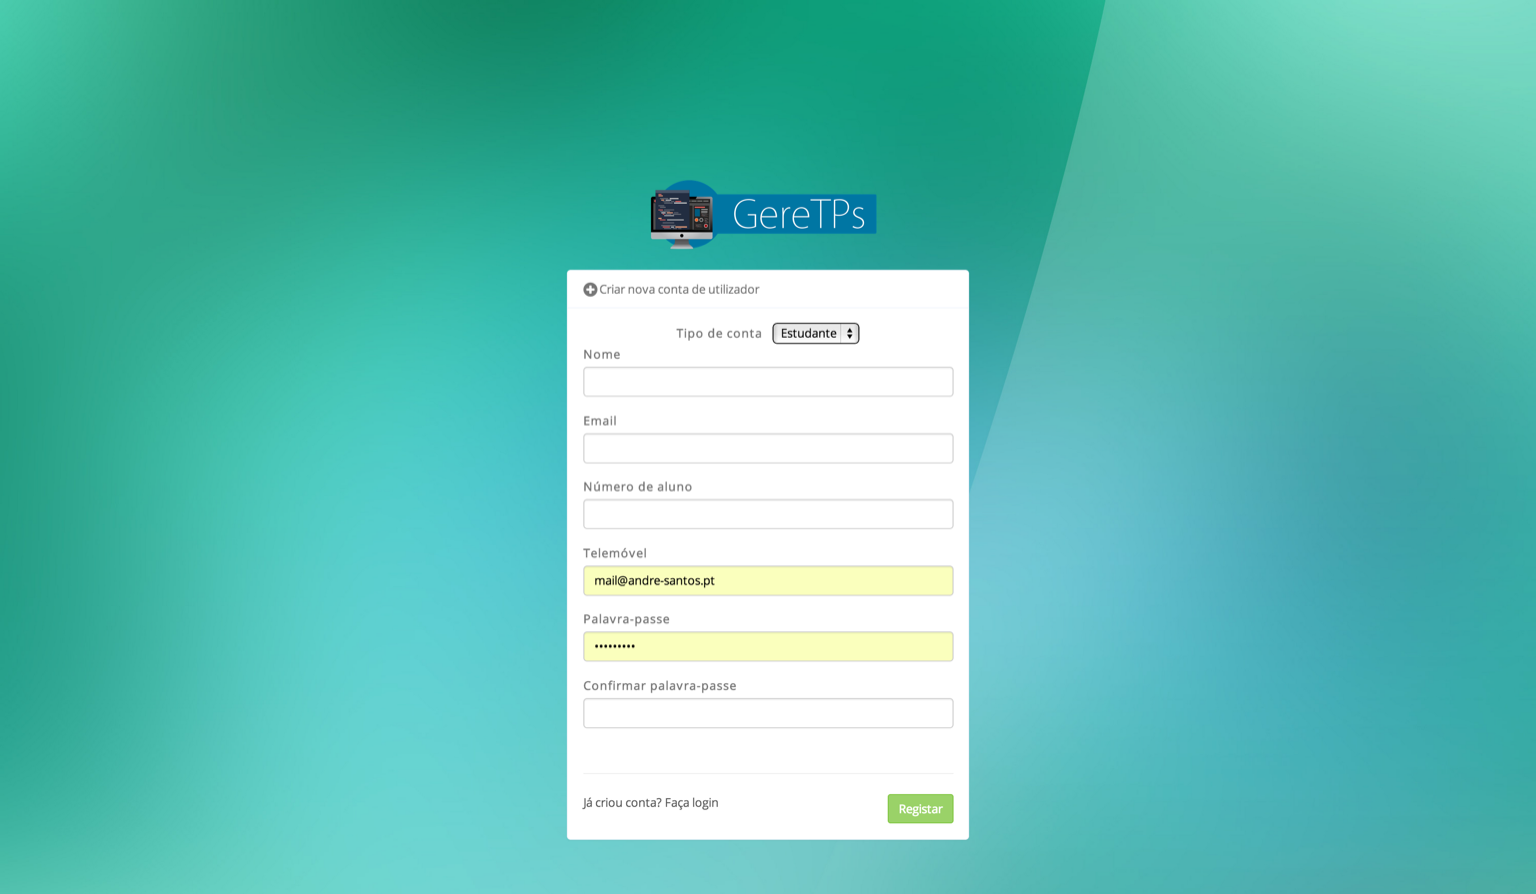
\includegraphics[width=1\textwidth,center]{images/implementacao/sign_up}
  \caption{Página de registo}
  \label{fig:sign_up}
\end{figure}
